% The working protocol

Nounce 64 bits long, Key 128 bits long.
The attacker can masquerade Alice, Bob, and Server.
The key distribution protocol is illustrated in \autoref{fig:nisec_protocol}.

\begin{figure}
    \centering

    \tikzset{every picture/.style={line width=0.75pt}} %set default line width to 0.75pt        

    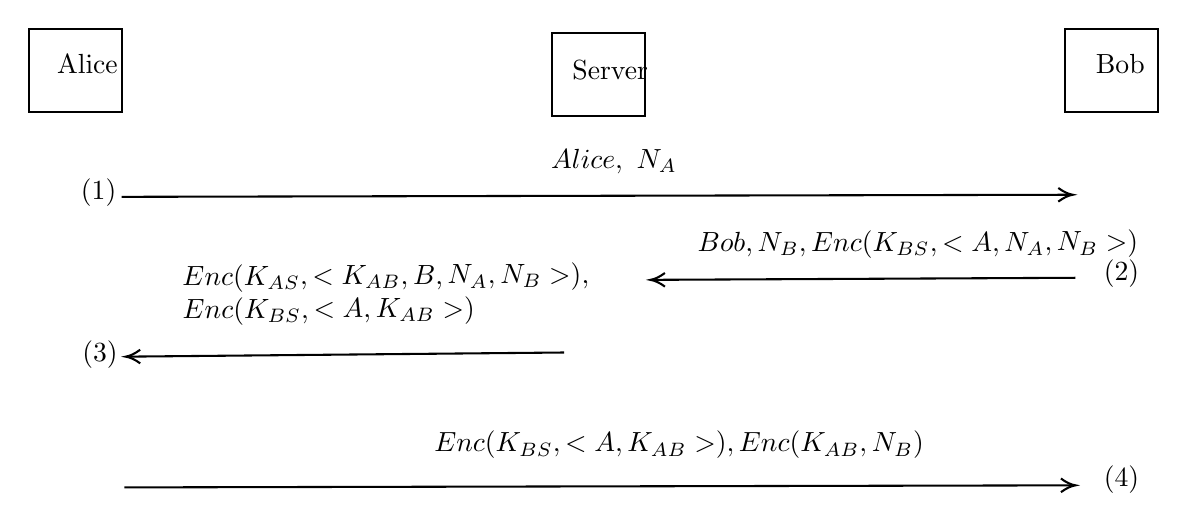
\begin{tikzpicture}[x=0.6pt,y=0.75pt,yscale=-1,xscale=0.8]
    %uncomment if require: \path (0,273); %set diagram left start at 0, and has height of 273

    %Shape: Rectangle [id:dp8079941464392838] 
    \draw   (43,29) -- (113,29) -- (113,69) -- (43,69) -- cycle ;

    %Shape: Rectangle [id:dp0032463221882207405] 
    \draw   (437,31) -- (507,31) -- (507,71) -- (437,71) -- cycle ;

    %Shape: Rectangle [id:dp9979101679316942] 
    \draw   (823,29) -- (893,29) -- (893,69) -- (823,69) -- cycle ;

    %Straight Lines [id:da824993271872942] 
    \draw    (113,110) -- (827,109) ;
    \draw [shift={(829,109)}, rotate = 179.92] [color={rgb, 255:red, 0; green, 0; blue, 0 }  ][line width=0.75]    (10.93,-3.29) .. controls (6.95,-1.4) and (3.31,-0.3) .. (0,0) .. controls (3.31,0.3) and (6.95,1.4) .. (10.93,3.29)   ;
    %Straight Lines [id:da5335074914742637] 
    \draw    (831,149) -- (513,149.99) ;
    \draw [shift={(511,150)}, rotate = 359.82] [color={rgb, 255:red, 0; green, 0; blue, 0 }  ][line width=0.75]    (10.93,-3.29) .. controls (6.95,-1.4) and (3.31,-0.3) .. (0,0) .. controls (3.31,0.3) and (6.95,1.4) .. (10.93,3.29)   ;
    %Straight Lines [id:da8549350781389543] 
    \draw    (446,185) -- (118,186.99) ;
    \draw [shift={(116,187)}, rotate = 359.65] [color={rgb, 255:red, 0; green, 0; blue, 0 }  ][line width=0.75]    (10.93,-3.29) .. controls (6.95,-1.4) and (3.31,-0.3) .. (0,0) .. controls (3.31,0.3) and (6.95,1.4) .. (10.93,3.29)   ;
    %Straight Lines [id:da35261899271615316] 
    \draw    (115,250) -- (829,249) ;
    \draw [shift={(831,249)}, rotate = 179.92] [color={rgb, 255:red, 0; green, 0; blue, 0 }  ][line width=0.75]    (10.93,-3.29) .. controls (6.95,-1.4) and (3.31,-0.3) .. (0,0) .. controls (3.31,0.3) and (6.95,1.4) .. (10.93,3.29)   ;

    % Text Node
    \draw (62,40) node [anchor=north west][inner sep=0.75pt]   [align=left] {Alice};
    % Text Node
    \draw (450,43) node [anchor=north west][inner sep=0.75pt]   [align=left] {Server};
    % Text Node
    \draw (844,40) node [anchor=north west][inner sep=0.75pt]   [align=left] {Bob};
    % Text Node
    \draw (434,85.4) node [anchor=north west][inner sep=0.75pt]    {$Alice,\ N_{A}$};
    % Text Node
    \draw (544.18,124.98) node [anchor=north west][inner sep=0.75pt]  [rotate=-359.86]  {$Bob,N_{B} ,Enc( K_{BS} ,< A,N_{A} ,N_{B}  >)$};
    % Text Node
    \draw (145.88,140.1) node [anchor=north west][inner sep=0.75pt]  [rotate=-359.66]  {$ \begin{array}{l}
    Enc( K_{AS} ,< K_{AB} ,B,N_{A} ,N_{B}  >) ,\\
    Enc( K_{BS} ,< A,K_{AB}  >)
    \end{array}$};
    % Text Node
    \draw (346,221.4) node [anchor=north west][inner sep=0.75pt]    {$Enc( K_{BS} ,< A,K_{AB}  >) ,Enc( K_{AB} ,N_{B})$};
    % Text Node
    \draw (850,139) node [anchor=north west][inner sep=0.75pt]   [align=left] {(2)};
    % Text Node
    \draw (850,238) node [anchor=north west][inner sep=0.75pt]   [align=left] {(4)};
    % Text Node
    \draw (80,100) node [anchor=north west][inner sep=0.75pt]   [align=left] {(1)};
    % Text Node
    \draw (81,178) node [anchor=north west][inner sep=0.75pt]   [align=left] {(3)};

    \end{tikzpicture}

    \caption{The new NISEC protocol.(Exercise 10)}\label{fig:nisec_protocol}

\end{figure}

%%%%%%%%%
%%%%%%%%% THE FIRST ATTACK
%%%%%%%%%

\subsection*{First attack --- Type flaw attack}
By utitlizing the length of session key is double the length of nounce, we
can trick Bob think that the session key \(K_{AB}=N_A||N_B\), where \(N_A\)
and \(N_B\) are publicly known. Message (3) is omitted and message (4) is
replaced by an attacker's version. The attack process is shown in \autoref{fig:type_flaw_attack}:

\begin{itemize}
    \item \(Alice \rightarrow Bob: Alice,N_A\)
    \item \(Bob \rightarrow Eve_{Server}: Bob,N_B,Enc(K_{BS},<A,N_A,N_B>)\)
    \item \(Eve_{Alice} \rightarrow Bob: Enc(K_{BS},<A,(N_A,N_B)=K'_{AB}>),
    Enc(K'_{AB},N_B)\)
\end{itemize}

\begin{figure}
    \centering

    \tikzset{every picture/.style={line width=0.75pt}} %set default line width to 0.75pt        

    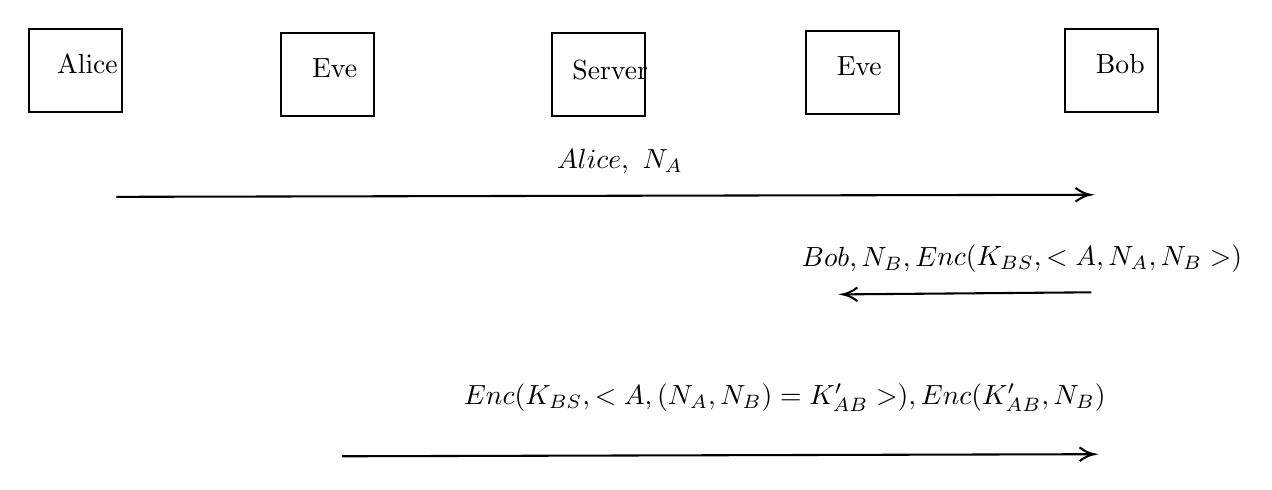
\begin{tikzpicture}[x=0.6pt,y=0.75pt,yscale=-1,xscale=0.8]
    %uncomment if require: \path (0,281); %set diagram left start at 0, and has height of 281

    %Shape: Rectangle [id:dp9386978289485048] 
    \draw   (63,49) -- (133,49) -- (133,89) -- (63,89) -- cycle ;

    %Shape: Rectangle [id:dp06671418882321467] 
    \draw   (457,51) -- (527,51) -- (527,91) -- (457,91) -- cycle ;

    %Shape: Rectangle [id:dp856946797480943] 
    \draw   (843,49) -- (913,49) -- (913,89) -- (843,89) -- cycle ;

    %Straight Lines [id:da2666329330469772] 
    \draw    (129,130) -- (860,129) ;
    \draw [shift={(862,129)}, rotate = 179.92] [color={rgb, 255:red, 0; green, 0; blue, 0 }  ][line width=0.75]    (10.93,-3.29) .. controls (6.95,-1.4) and (3.31,-0.3) .. (0,0) .. controls (3.31,0.3) and (6.95,1.4) .. (10.93,3.29)   ;

    %Straight Lines [id:da6152100696793793] 
    \draw    (862.9,176) -- (677.96,176.99) ;
    \draw [shift={(675.96,177)}, rotate = 359.69] [color={rgb, 255:red, 0; green, 0; blue, 0 }  ][line width=0.75]    (10.93,-3.29) .. controls (6.95,-1.4) and (3.31,-0.3) .. (0,0) .. controls (3.31,0.3) and (6.95,1.4) .. (10.93,3.29)   ;

    %Shape: Rectangle [id:dp04492139578009846] 
    \draw   (253,51) -- (323,51) -- (323,91) -- (253,91) -- cycle ;

    %Straight Lines [id:da054736882600693315] 
    \draw    (299,255) -- (863,254) ;
    \draw [shift={(865,254)}, rotate = 179.9] [color={rgb, 255:red, 0; green, 0; blue, 0 }  ][line width=0.75]    (10.93,-3.29) .. controls (6.95,-1.4) and (3.31,-0.3) .. (0,0) .. controls (3.31,0.3) and (6.95,1.4) .. (10.93,3.29)   ;
    %Shape: Rectangle [id:dp4939998903404802] 
    \draw   (648,50) -- (718,50) -- (718,90) -- (648,90) -- cycle ;


    % Text Node
    \draw (864,60) node [anchor=north west][inner sep=0.75pt]   [align=left] {Bob};
    % Text Node
    \draw (470,63) node [anchor=north west][inner sep=0.75pt]   [align=left] {Server};
    % Text Node
    \draw (82,60) node [anchor=north west][inner sep=0.75pt]   [align=left] {Alice};
    % Text Node
    \draw (642.52,151.98) node [anchor=north west][inner sep=0.75pt]  [rotate=-359.86]  {$Bob,N_{B} ,Enc( K_{BS} ,< A,N_{A} ,N_{B}  >)$};
    % Text Node
    \draw (458.49,105.4) node [anchor=north west][inner sep=0.75pt]    {$Alice,\ N_{A}$};
    % Text Node
    \draw (274,62) node [anchor=north west][inner sep=0.75pt]   [align=left] {Eve};
    % Text Node
    \draw (388.27,218.4) node [anchor=north west][inner sep=0.75pt]    {$Enc( K_{BS} ,< A,( N_{A} ,N_{B}) =K'_{AB}  >) ,Enc( K'_{AB} ,N_{B})$};
    % Text Node
    \draw (669,61) node [anchor=north west][inner sep=0.75pt]   [align=left] {Eve};


    \end{tikzpicture}

    \caption{Type flaw attack.(Exercise 10)}\label{fig:type_flaw_attack}

\end{figure}

%%%%%%%%% THE FIRST COUNTERMEASURE

\subsubsection*{Countermeasure}
We can avoid the above attack by adding the new field \(N_B\) in the message (3), (4)
as shown in the \autoref{fig:countermeasure_tf_attack}. By adding the field nounce \(N_B\)
, \(Enc(K_{BS},<A,K_{AB},N_B>)\) now has 3 fields where \(K_{AB}\) 128-bits long and \(
N_B\) 64-bits long. Thus, the attacker cannot replace it by \(Enc(K_{BS},<A,N_A,N_B>)\)
in which \(N_A\) and \(N_B\) both 64-bits long.

\begin{figure}
    \centering

    \tikzset{every picture/.style={line width=0.75pt}} %set default line width to 0.75pt        

    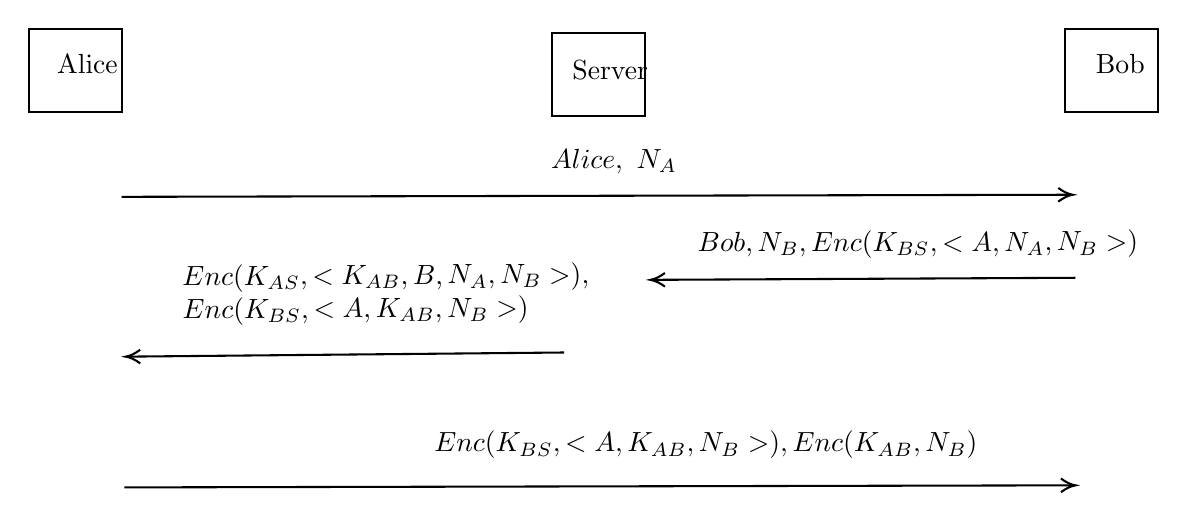
\begin{tikzpicture}[x=0.6pt,y=0.75pt,yscale=-1,xscale=0.8]
    %uncomment if require: \path (0,300); %set diagram left start at 0, and has height of 300

    %Shape: Rectangle [id:dp4526236491151884] 
    \draw   (63,49) -- (133,49) -- (133,89) -- (63,89) -- cycle ;

    %Shape: Rectangle [id:dp10175097601664151] 
    \draw   (457,51) -- (527,51) -- (527,91) -- (457,91) -- cycle ;

    %Shape: Rectangle [id:dp5837028242450013] 
    \draw   (843,49) -- (913,49) -- (913,89) -- (843,89) -- cycle ;

    %Straight Lines [id:da18293032398791997] 
    \draw    (133,130) -- (847,129) ;
    \draw [shift={(849,129)}, rotate = 179.92] [color={rgb, 255:red, 0; green, 0; blue, 0 }  ][line width=0.75]    (10.93,-3.29) .. controls (6.95,-1.4) and (3.31,-0.3) .. (0,0) .. controls (3.31,0.3) and (6.95,1.4) .. (10.93,3.29)   ;
    %Straight Lines [id:da18962783133023287] 
    \draw    (851,169) -- (533,169.99) ;
    \draw [shift={(531,170)}, rotate = 359.82] [color={rgb, 255:red, 0; green, 0; blue, 0 }  ][line width=0.75]    (10.93,-3.29) .. controls (6.95,-1.4) and (3.31,-0.3) .. (0,0) .. controls (3.31,0.3) and (6.95,1.4) .. (10.93,3.29)   ;
    %Straight Lines [id:da09963880475389586] 
    \draw    (466,205) -- (138,206.99) ;
    \draw [shift={(136,207)}, rotate = 359.65] [color={rgb, 255:red, 0; green, 0; blue, 0 }  ][line width=0.75]    (10.93,-3.29) .. controls (6.95,-1.4) and (3.31,-0.3) .. (0,0) .. controls (3.31,0.3) and (6.95,1.4) .. (10.93,3.29)   ;
    %Straight Lines [id:da9372056196507472] 
    \draw    (135,270) -- (849,269) ;
    \draw [shift={(851,269)}, rotate = 179.92] [color={rgb, 255:red, 0; green, 0; blue, 0 }  ][line width=0.75]    (10.93,-3.29) .. controls (6.95,-1.4) and (3.31,-0.3) .. (0,0) .. controls (3.31,0.3) and (6.95,1.4) .. (10.93,3.29)   ;

    % Text Node
    \draw (454,105.4) node [anchor=north west][inner sep=0.75pt]    {$Alice,\ N_{A}$};
    % Text Node
    \draw (564.18,144.98) node [anchor=north west][inner sep=0.75pt]  [rotate=-359.86]  {$Bob,N_{B} ,Enc( K_{BS} ,< A,N_{A} ,N_{B}  >)$};
    % Text Node
    \draw (165.88,160.1) node [anchor=north west][inner sep=0.75pt]  [rotate=-359.66]  {$ \begin{array}{l}
    Enc( K_{AS} ,< K_{AB} ,B,N_{A} ,N_{B}  >) ,\\
    Enc( K_{BS} ,< A,K_{AB} ,N_{B}  >)
    \end{array}$};
    % Text Node
    \draw (366,241.4) node [anchor=north west][inner sep=0.75pt]    {$Enc( K_{BS} ,< A,K_{AB} ,N_{B}  >) ,Enc( K_{AB} ,N_{B})$};
    % Text Node
    \draw (864,60) node [anchor=north west][inner sep=0.75pt]   [align=left] {Bob};
    % Text Node
    \draw (470,63) node [anchor=north west][inner sep=0.75pt]   [align=left] {Server};
    % Text Node
    \draw (82,60) node [anchor=north west][inner sep=0.75pt]   [align=left] {Alice};

    \end{tikzpicture}


    \caption{Countermeasure of type flaw attack.(Exercise 10)}\label{fig:countermeasure_tf_attack}

\end{figure}

%%%%%%%%%
%%%%%%%%% THE SECOND ATTACK
%%%%%%%%%

\subsection*{Second attack --- Replay attack}
The attacker can use the old session key \(K'_{AB}\) which was compromised so that replace the
message (4) by its own his/her message. Moreover, the nounce \(N_B\) is public, so
the attacker can encrypt it using the leaked session key and include it in his/her
own message (4) for authenticating. The attack process is shown in \autoref{fig:replay_attack}:

\begin{itemize}
    \item \(Alice \rightarrow Bob: Alice,N_A\)
    \item \(Bob \rightarrow Eve_{Server}: Bob,N_B,Enc(K_{BS},<A,N_A,N_B>)\)
    \item \(Eve_{Alice} \rightarrow Bob: Enc(K_{BS},<A,K'_{AB}>),Enc(K'_{AB},N_B)\)
\end{itemize}

\begin{figure}
    \centering

    \tikzset{every picture/.style={line width=0.75pt}} %set default line width to 0.75pt        

    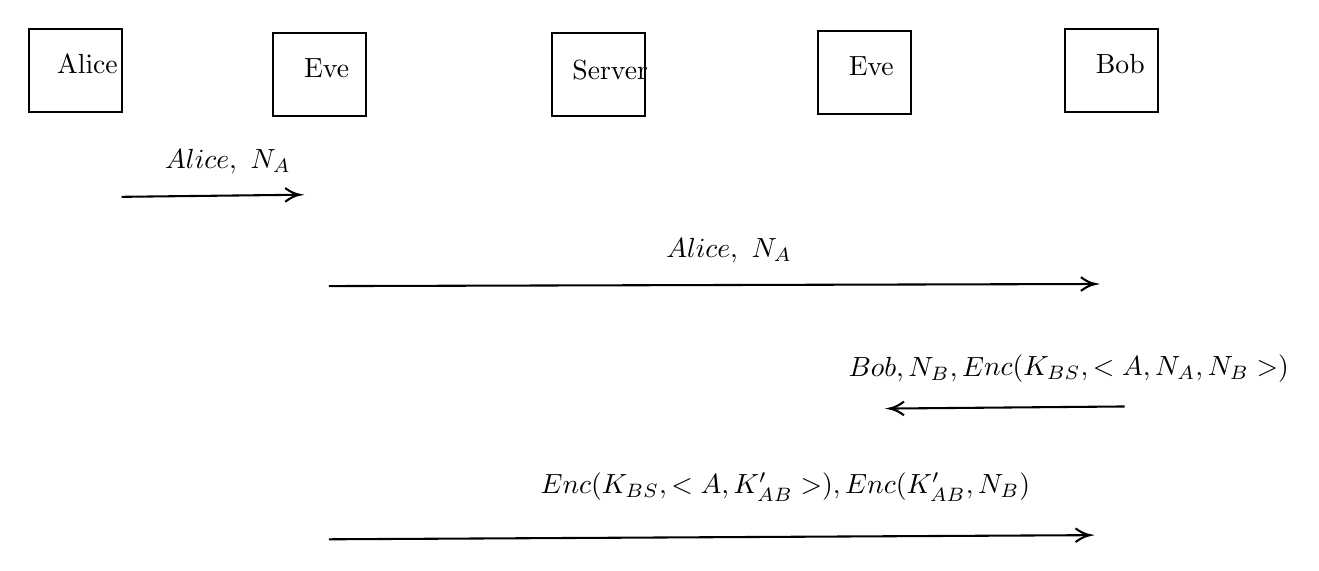
\begin{tikzpicture}[x=0.6pt,y=0.75pt,yscale=-1,xscale=0.8]
    %uncomment if require: \path (0,307); %set diagram left start at 0, and has height of 307

    %Shape: Rectangle [id:dp15812126315922326] 
    \draw   (63,32) -- (133,32) -- (133,72) -- (63,72) -- cycle ;

    %Shape: Rectangle [id:dp7720928287797268] 
    \draw   (457,34) -- (527,34) -- (527,74) -- (457,74) -- cycle ;

    %Shape: Rectangle [id:dp478327433731622] 
    \draw   (843,32) -- (913,32) -- (913,72) -- (843,72) -- cycle ;

    %Straight Lines [id:da006883984521392605] 
    \draw    (133,113) -- (265,112.01) ;
    \draw [shift={(267,112)}, rotate = 179.57] [color={rgb, 255:red, 0; green, 0; blue, 0 }  ][line width=0.75]    (10.93,-3.29) .. controls (6.95,-1.4) and (3.31,-0.3) .. (0,0) .. controls (3.31,0.3) and (6.95,1.4) .. (10.93,3.29)   ;
    %Straight Lines [id:da007102795315477861] 
    \draw    (888,214) -- (713,214.99) ;
    \draw [shift={(711,215)}, rotate = 359.68] [color={rgb, 255:red, 0; green, 0; blue, 0 }  ][line width=0.75]    (10.93,-3.29) .. controls (6.95,-1.4) and (3.31,-0.3) .. (0,0) .. controls (3.31,0.3) and (6.95,1.4) .. (10.93,3.29)   ;
    %Straight Lines [id:da3936689672070055] 
    \draw    (289,278) -- (860,276.01) ;
    \draw [shift={(862,276)}, rotate = 179.8] [color={rgb, 255:red, 0; green, 0; blue, 0 }  ][line width=0.75]    (10.93,-3.29) .. controls (6.95,-1.4) and (3.31,-0.3) .. (0,0) .. controls (3.31,0.3) and (6.95,1.4) .. (10.93,3.29)   ;
    %Shape: Rectangle [id:dp7524914360610107] 
    \draw   (247,34) -- (317,34) -- (317,74) -- (247,74) -- cycle ;

    %Straight Lines [id:da5224935211148828] 
    \draw    (289,156) -- (864,155) ;
    \draw [shift={(866,155)}, rotate = 179.9] [color={rgb, 255:red, 0; green, 0; blue, 0 }  ][line width=0.75]    (10.93,-3.29) .. controls (6.95,-1.4) and (3.31,-0.3) .. (0,0) .. controls (3.31,0.3) and (6.95,1.4) .. (10.93,3.29)   ;
    %Shape: Rectangle [id:dp8247419138301741] 
    \draw   (657,33) -- (727,33) -- (727,73) -- (657,73) -- cycle ;


    % Text Node
    \draw (163.41,88.4) node [anchor=north west][inner sep=0.75pt]    {$Alice,\ N_{A}$};
    % Text Node
    \draw (677.76,187.98) node [anchor=north west][inner sep=0.75pt]  [rotate=-359.86]  {$Bob,N_{B} ,Enc( K_{BS} ,< A,N_{A} ,N_{B}  >)$};
    % Text Node
    \draw (446,244.4) node [anchor=north west][inner sep=0.75pt]    {$Enc( K_{BS} ,< A,K'_{AB}  >) ,Enc( K'_{AB} ,N_{B})$};
    % Text Node
    \draw (864,43) node [anchor=north west][inner sep=0.75pt]   [align=left] {Bob};
    % Text Node
    \draw (470,46) node [anchor=north west][inner sep=0.75pt]   [align=left] {Server};
    % Text Node
    \draw (82,43) node [anchor=north west][inner sep=0.75pt]   [align=left] {Alice};
    % Text Node
    \draw (268,45) node [anchor=north west][inner sep=0.75pt]   [align=left] {Eve};
    % Text Node
    \draw (540.6,131.4) node [anchor=north west][inner sep=0.75pt]    {$Alice,\ N_{A}$};
    % Text Node
    \draw (678,44) node [anchor=north west][inner sep=0.75pt]   [align=left] {Eve};

    \end{tikzpicture}


    \caption{Replay attack --- an old session key was leaked.(Exercise 10)}\label{fig:replay_attack}
\end{figure}

%%%%%%%%% THE SECOND COUNTERMEASURE

\subsubsection*{Countermeasure}
In the \autoref{fig:countermeasure_tf_attack}, the nounce \(N_B\) is encrypted
,and it is included in the certificate containing session key \(Enc(K_{BS}, 
<A,K_{AB},N_B>)\). Thus, even other keys or nounces are compromised, the attacker
cannot authenticate himself without knowing the secret nounce \(N_B\).